\section{Α.Α.Μ. σε βάθος}
Ο Αλγόριθμος Αποικίας Μυρμηγκιών (Α.Α.Μ.) είναι ένας μετευρετικός αλγόριθμος βελτιστοποίησης που έχει ως στόχο την εύρεσης βέλτιστης διαδρομής σε κάποιο πρόβλημα. Μετευρετικούς ονομάζουμε τους αλγόριθμους που είναι βασισμένοι σε ευφυείς επαναληπτικές τεχνικές και αντί να ακουλουθούν έναν αυστηρό κανόνα εξάγουν γνώση με τρόπους που είναι εμπνευσμένοι από συμπεριφορές στην φύση. \cite{Maniezzo} Συγκεκριμένα, ο Α.Α.Μ. είναι βασισμένος στην συμπεριφορά τον μυρμηγκιών για την αναζήτηση τροφής. 
Τα μυρμήγκια έχουν την ικανότητα να βρίσκουν πάντα την βέλτιστη διαδρομή προς την πηγή τροφής όσο δύσκολο κι αν είναι αυτό. Κατά συνέπεια κι ο Α.Α.Μ. είναι ικανός να βρει ικανοποιητικές λύσεις σε περίπλοκα προβλήματα και να εξερευνήσει μεγάλους χώρους αναζήτησης σε μικρό χρονικό διάστημα. Όπως αναφέρθηκε και στο προηγούμενο κεφάλαιο, όταν τα μυρμήγκια κινούνται στο χώρο αφήνουν φερομόνη. Αυτή η ουσία αποτελεί και τρόπο επικοινωνίας μεταξύ των μυρμηγκιών, για εύρεση βέλτιστης διαδρομής προς την τροφή, αφού όσο περισσότερη φερομόνη υπάρχει σε μία διαδρομή, τόσο αυξάναται κι η πιθανότητα ένα επόμενο μυρμήγκι να ακολουθήσει αυτή τη διαδρομή. 

\subsection{Βασική Θεωρία}
Τα τεχνητά μυρμήγκια που χρησιμοποιούνται στον Α.Α.Μ. είναι εμπνευσμένα από την συμπεριφορά των πραγματικών μυρμηγκιών και αποτελούν διαδικασίες κατασκευής στοχαστικών λύσεων που με χρήση πιθανολογικών τεχνικών επιλύουν υπολογιστικά προβλήματα, όπως αυτό της εύρεσης βέλτιστου μονοπατιού μέσω γράφων, προσθέτοντας επαναληπτικά στοιχεία σε επιμέρους λύσεις λαμβάνοντας υπόψη ευρετικές πληροφορίες σχετικά με την επίλυση του προβλήματος και (τεχνητές) διαδρομές φερομόνης που αλλάζουν δυναμικά στο χρόνο εκτέλεσης. \cite{Dorigo-Stutzle}

\subsection{Μαθηματικό υπόβαθρο}


\begin{figure}[ht]
    \begin{minipage}[c]{.46\linewidth}
        \centering
        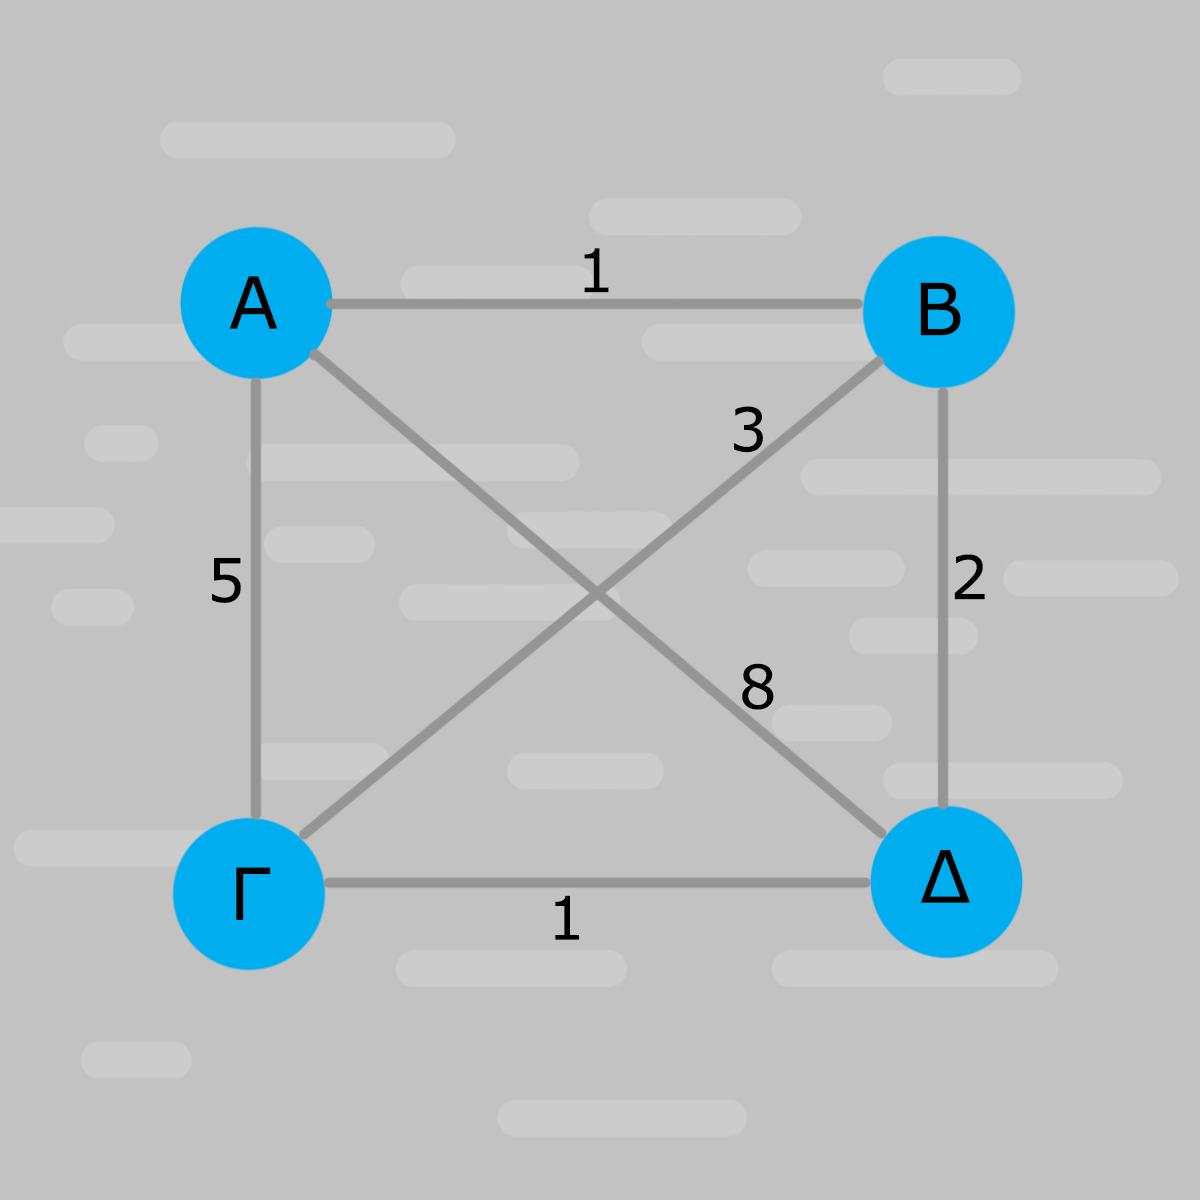
\includegraphics[scale=0.15]{2947_thesis/pictures/apostaseis.png}
        \caption{Απόσταση}
    \end{minipage}
    \begin{minipage}[c]{.46\linewidth}
        \centering
        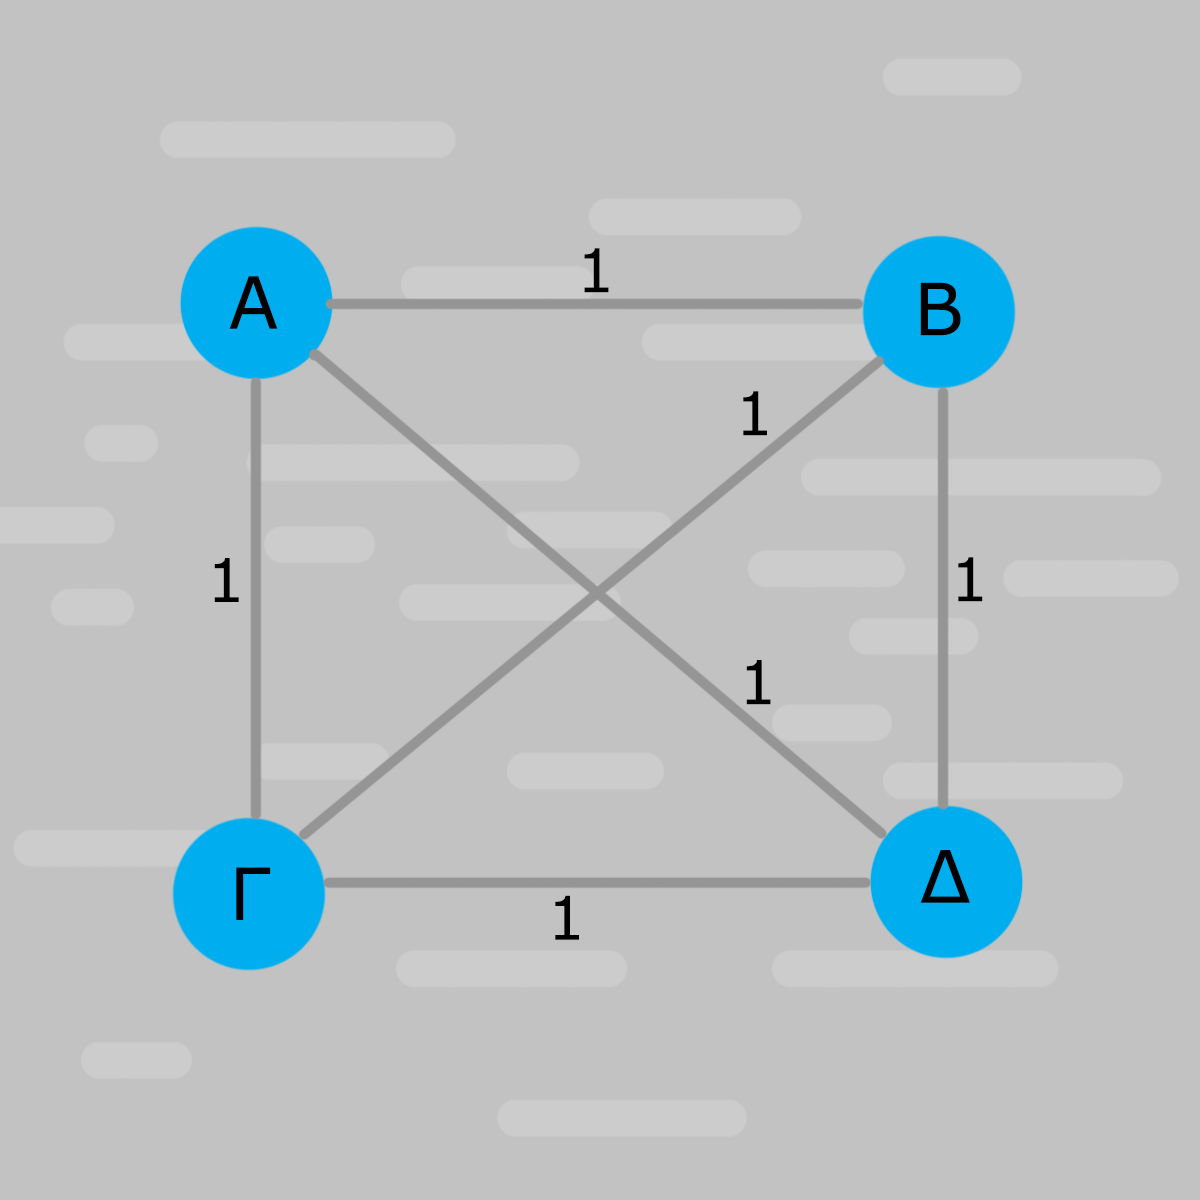
\includegraphics[scale=0.15]{2947_thesis/pictures/feromoni.png}
        \caption{Φερομόνη}
    \end{minipage}
\end{figure}
\subsubsection{Απόσταση}
Όπως αναφέρθηκε και στην δεύτερη ενότητα, ο γράφος είναι ένα απαραίτητο κομμάτι για τη μοντελοποίηση προβλημάτων με χρήση του αλγόριθμου αποικίας μυρμηγκιών. Η απόσταση, όπως και η φερομόνη, θα μοντελοποιηθούν με χρήση αναπαράστασης πίνακα. Κάθε ακμή του γράφο έχει ένα κόστος που συμβολίζει την απόσταση ή την γενικότερη ποιότητα της διαδρομής μεταξύ δύο κορυφών. Έστω οι κορυφές Α, Β, Γ, Δ που ενώνονται μεταξύ τους όπως φαίνεται στο [Σχήμα 8] το οποίο αποτυπώνεται σε πίνακα γειτνίασης ως εξής:
$$
Distance = 
 \begin{array}{c|c c c c}
    & A & B & Γ & Δ \\ \hline
    A & 0 & 1 & 8 & 5 \\
    B & 1 & 0 & 2 & 3 \\
    Γ & 8 & 2 & 0 & 1 \\
    Δ & 5 & 3 & 1 & 0 
 \end{array}
 $$
\subsubsection{Φερομόνη}
Τα μυρμήγκια αφήνουν φερομόνη από όπου περνούν ανάλογα από την ποιότητα της λύσης που βρήκαν ώστε να γνωρίζουν τα επόμενα. Τα μονοπάτια φερομόνης χρησιμεύουν ως αριθμητικές πληροφορίες που χρησιμοποιούν τα μυρμήγκια για να κατασκευάσουν πιθανές λύσεις στο εκάστοτε πρόβλημα και τα οποία μεταβάλονται κατά την εκτέλεση του αλγορίθμου με στόχο της εύρεση του βέλτιστου μονοπατιού. \cite{Dorigo-Stutzle} Σε μονοπάτια που το μυρμήγκι θα έχει επιστρέψει σε σύντομο χρονικό διάστημα συσσωρεύεται περισσότερη φερομόνη από άλλα μονοπάτια. Υπάρχουν μοντέλα που παράγωγουν περισσότερη φερομόνη ανάλογα με την ποιότητα αυτής της διαδρομής (για παράδειγμα την απόσταση, την ποσότητα της τροφής, και άλλα)
 
Το μαθηματικό μοντέλο αναπαράστασης της φερομόνης που εξάγει το κ-οστό μυρμήγκι στην ακμή που ενώνει τις κορυφές i και j (δηλαδή η ποσότητα της φερομόνης που παράγει) είναι αντιστρόφος ανάλογη με την απόσταση και προκύπτει από τον τύπο:

\begin{align}
	Δτ^k_{i,j}=\frac{1}{L_k}
\end{align}
Όπου:
\begin{itemize}
    \item $L_k$: Η ποιότητα της διαδρομής που βρήκε το μυρμήγκι
\end{itemize}
Έστω ότι για το πρώτο μυρμήγκι είναι παντού 1 [Σχήμα 9]. Με αποτέλεσμα να είναι τυχαία η επιλογή διαδρομής. Στο παράδειγμα μας προκύπτει ο πίνακας: 
$$
Pheromone = 
 \begin{array}{c|c c c c}
    & A & B & Γ & Δ \\ \hline
    A & 0 & 1 & 1 & 1 \\
    B & 1 & 0 & 1 & 1 \\
    Γ & 1 & 1 & 0 & 1 \\
    Δ & 1 & 1 & 1 & 0 
 \end{array}
 $$
Οπότε ως έδώ έχουμε ένα χάρτη με τις πιθανά μονοπάτια στον πίνακα distance και το αντίστοιχο κόστος της κάθε διαδρομής και έναν ακόμα με την "επιθυμία" του μυρμηγκιού να επιλέγει το κάθε μονοπάτι στον πίνακα pheromone.

Για να υπολογίσουμε την ποσότητα φερομόνης από μια κορυφή σε μία άλλη (χωρίς εξασθένση- θα αναλυθεί παρακάτω) υπολογίζουμε το άθροισμα της φερομόνης που εξήγαγαν τα μυρμήγκια m που πέρασαν από την κορυφή i στην j. Δηλαδή: 
\begin{align}
    τ_{i,j}^k=\sum_{k=1}^{m}{Δτ^k_{i,j}}
\end{align}

\begin{figure}
    \centering
    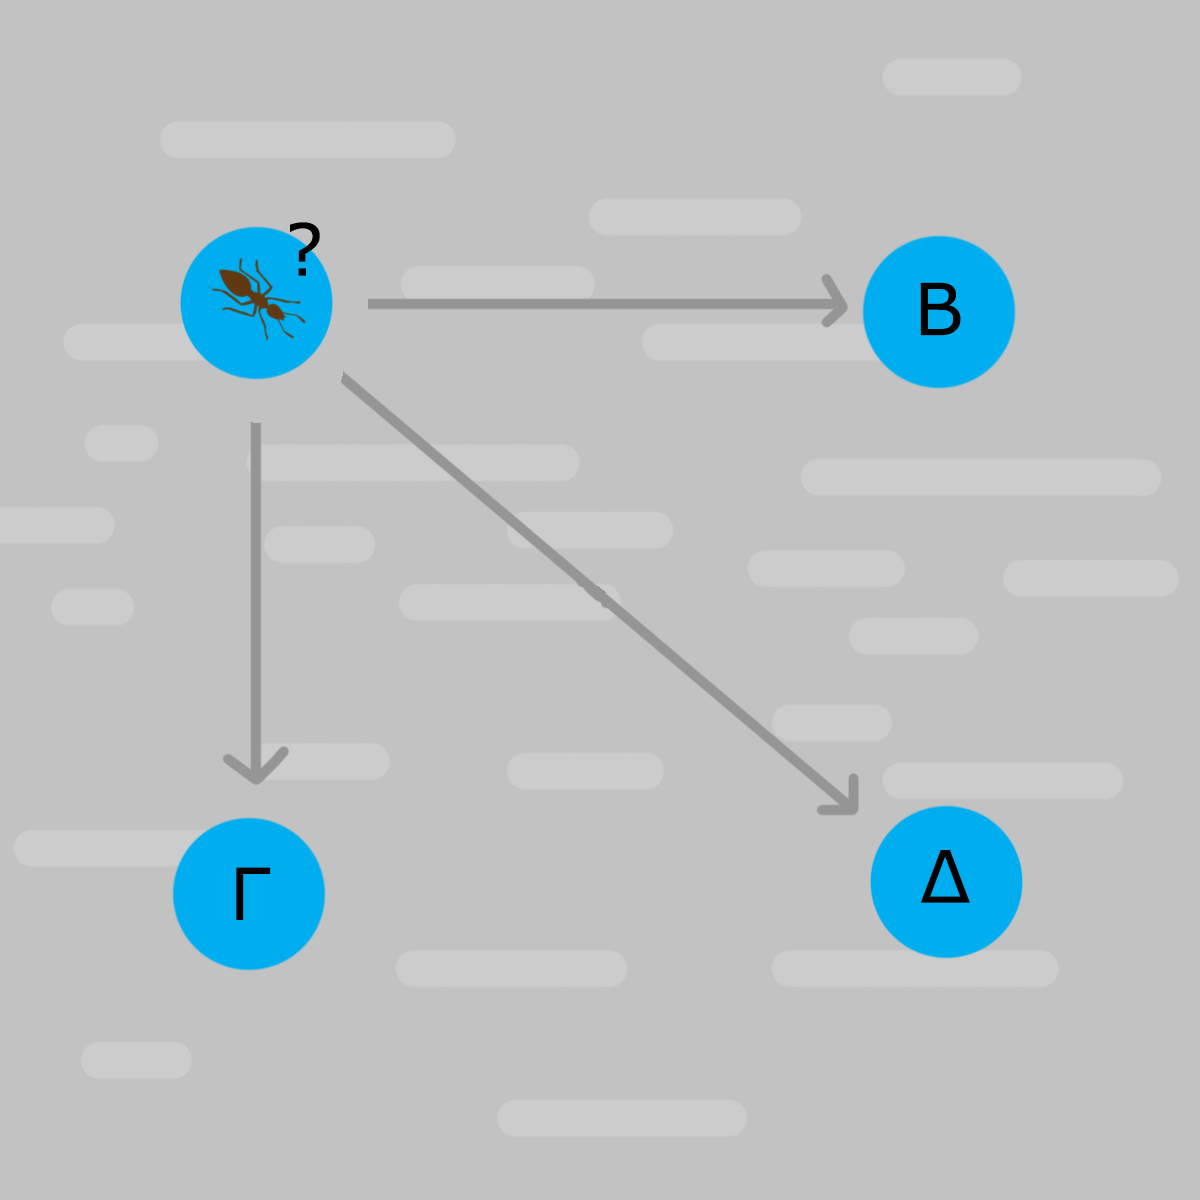
\includegraphics[scale=0.20]{2947_thesis/pictures/epilogi.png} 
    \caption{Πιθανές επιλογές}
\end{figure}

\subsubsection{Επιλογή Διαδρομής}
Στο παράδειγμα μας ας υποθέσουμε ότι ένα μυρμήγκι ξεκινάει στην κορυφή Α. Οι πιθανές του επιλογές όπως φαίνεται και στο [Σχήμα 10] είναι οι Β, Γ, Δ. Ποιά είναι όμως η βέλτιστη; 
Με το μάτι σε ένα τόσο απλό πρόβλημα είναι εύκολο να αντιληφθούμε ποιά διαδρομή πρέπει να ακολουθήσει το μυρμήγκι, όμως αυτό δεν είναι εφικτό σε πιο περίπλοκα προβλήματα με μεγάλο αριθμό κορυφών. Έστω ότι ο αριθμός των κορυφών είναι n τότε επιλέγοντας μία κορυφη ως αρχική ο αριθμός των πιθανών κορυφών γίνεται n-1. Αφού το μυρμήγκι επιλέξει μία από αυτή μετά θα αφαιρεθεί από τις πιθανές αφού επισκέφθηκε και θα γίνουν n-2. Έτσι θα επιλέγει μονοπάτια μεχρι να μην μείνει κανένα διαθέσιμο και να επιστρέψει στο αρχικό. Άρα ο αριθμός των πιθανών επιλογών είναι (n-1)(n-2)(n-3)...3*2*1 = (n-1)!. Όμως δεδομένου ότι διαδρομές όπως Α->Β->Γ->Δ->Α είναι ίδια με την Α->Δ->Γ->Β->Α. Οπότε αφού πρόκειται για συμμετρικό πρόβλημα ο τύπος αριθμός των πιθανών μονοπατιών γίνεται (n-1)!/2 αφαιρώντας τις επαναλαμβανόμενες λύσεις όπως και στο πρόβλημα του πλανόδιου πωλητή. 
Η πιθανότητα το κ-οστό μυρμήγκι να επιλέξει μια διαδρομή συμβολίζεται ως: $P^k_{i,j}$ και δίνεται από τον τύπο: \cite{CPVBK}

\begin{align}
	P^k_{i,j}=\frac{(τ_{i,j})^α(η_{i,j})^β}{\sum_{m}(τ_{i,m})^α(η_{i,m})^β}
\end{align}

Όπου: 
\begin{itemize}
    \item $τ_{i,j}$: το επίπεδο φερομόνης μεταξύ των κορυφών i και j
    \item $η_{i,j}$: είναι η ποιότητα της διαδρομής
    \item m: η υπόλοιπες διαδρομές που μπορούσε να επιλέξει το μυρμήγκι
    \item α, β: σταθερές που επιλέγουμε ανάλογα από την επιρροή που θέλουμε να έχει το τ και το η στην διαδικασία επιλογής. (Για παράδειγμα αν θέλουμε να επιλέξουμε μια διαδρομή βασισμένη αποκλιστικά και μόνο στο επίπεδο της φερομόνης τότε αφαιρούμε από την εξίσοση το $η_{i,j}$ θέτοντας το β=0).
\end{itemize}
Το γινόμενο των $τ_{i,j}*η_{i,j}$ μας δίνει την "επιθυμία" του μυρμηγκιού να επιλέξει το μονοπάτι i,j.
Στις περισσότερες βιβλιογραφίες αυτή η πιθανότητα αναφέρετε έτσι με διαφορετικούς συμβολισμούς στην καθεμία. 

Στο παράδειγμα μας, αφού υπολογίσουμε την επιθυμία του μυρμηγκιού να επιλέξει την κάθε διαδρομή έχουμε:

\begin{itemize}
    \item Α->Β = $τ_{Α,Β}η_{Α,Β}=1*\frac{1}{1}=1$ 
    \item Α->Γ = $τ_{Α,Γ}η_{Α,Γ}=1*\frac{1}{5}=0.2$
    \item Α->Δ = $τ_{Α,Δ}η_{Α,Δ}=1*\frac{1}{8}=0.125$
\end{itemize}

Όπου οι αντίστοιχες πιθανότητες γίνονται:

\begin{itemize}
    \item $P_{A,B}=\frac{1}{1+0.125+0.2}=\frac{1}{1.325}=0.76$
    \item $P_{Α,Γ}=\frac{0.2}{1.325}=0.15$
    \item $P_{A,Δ}=\frac{0.125}{1.325}=0.09$
\end{itemize}

Βλέπουμε ότι πιο πιθανό είναι το μυρμήγκι να επιλέξει την διαδρομή ΑΒ όμως υπάρχει πιθανότητα να επιλέξει και τις υπόλοιπες, για να προσομοιώσουμε την τυχαία επιλογή μονοπατιού με βάση την πιθανότητα χρησιμοποιούμε την τεχνική roulette wheel \cite{Adam-Dorota}, όπου υπολογίζουμε το άθροισμα συσσωρευμένο, αφού πρόκειτε για πιθανότητα το άθροισμα τους είναι 1, γίνεται η τυχαία επιλογή ενός αριθμού από το 0 έως το 1 και βρίσκουμε το σύνολο στο οποίο αντιστοιχεί αυτός ο αριθμός. Στο παράδειγμά μας από 0 έως 0,76 αντιστοιχεί στην διαδρομή ΑΒ, από το 0,77 εως το 0,91 αντιστοιχεί στην διαδρομή ΑΓ και απο το 0,92 έως το 1 στην διαδρομή ΑΔ. Όποτε αν για παράδειγμα επιλεγόταν ο αριθμός 0,56 θα πηγαίναμε στην διαδρομή ΑΒ.

\subsubsection{Εξασθένιση Φερομόνης}
(4.2.2 αναφέρθηκε)

\subsection{Υλοποίησή μου Αλγορίθμου σε python}
(4.2.3 τυχαία επιλογή αριθμού από τις πιθανότητες)

\subsection{Εφαρμογές Αλγόριθμου}
Θα δωθούν  προβλήματα πραγματικού κόσμου που λύνει αυτός ο αλγόριθμος

\subsection{Βελτιστοποίηση Αλγόριθμου}
